\documentclass[a4paper, 12pt]{article}
\usepackage[T2A]{fontenc}
\usepackage[utf8]{inputenc}
\usepackage[english,russian]{babel}
\usepackage{titletoc}
\usepackage{graphicx}
\usepackage{array}
\usepackage{etoolbox}
\usepackage{subfig}
\newcolumntype{P}[1]{>{\centering\arraybackslash}p{#1}}
\def\textunderset#1#2{\leavevmode
  \vtop{\offinterlineskip\halign{%
    \hfil##\hfil\cr\strut#2\cr\noalign{\kern-.3ex}
    \hidewidth\strut#1\hidewidth\cr}}}
\def\signhrule{\raggedright\baselineskip30.0ex \vrule height 0.5pt width30mm depth0pt}


\dottedcontents{section}[2.5em]{\bfseries}{2em}{0.5pc}
\dottedcontents{subsection}[3em]{}{2em}{0.5pc}

\usepackage{hyperref}
\hypersetup{
    colorlinks=true, %set true if you want colored links
    linktoc=all,     %set to all if you want both sections and subsections linked
    linkcolor=black,  %choose some color if you want links to stand out
}

\usepackage{verbatim}

\usepackage{listings}
\usepackage{xcolor}

\lstset
{%
	extendedchars=\true,
	inputencoding=utf8x,
	keepspaces=true,
	frame=tb,
	escapechar=|,
	xleftmargin=0.5cm,
	xrightmargin=0.5cm,
	columns=fullflexible,
	numbers=left,
	numbersep=4pt,
	showspaces=false,
	showstringspaces=false,
	breakatwhitespace=true,
	breaklines=true,
	basicstyle=\color{black}\small\sffamily,
	commentstyle=\color{gray}\itshape,
	stringstyle=\color{orange},
	numberstyle=\footnotesize\color{gray},
	keywordstyle=\color{blue}\bfseries,
	emphstyle={\color{blue}\bfseries},
	tabsize=2,
	texcl=true,
}

\lstdefinestyle{text}{
basicstyle=\small\ttfamily,
columns=flexible,
breaklines=true,
breakatwhitespace=true,
literate={\-}{{-\allowbreak}}1,
numbers=none,
postbreak=\mbox{\textcolor{red}{$\hookrightarrow$}\space},
}

\lstloadlanguages{SQL}

\newcommand{\Title}{Отчет о выполнении лабораторной работы}
\newcommand{\TaskType}{лабораторная работа}
\newcommand{\SubTitle}{по дисциплине <<Поддержка принятия решений в системах мониторинга>>}
\newcommand{\LabTitle}{Выявление логических закономерностей по данным мониторинга} 
\newcommand{\Faculty}{<<Информатика и системы управления>>}
\newcommand{\Department}{<<Компьютерные системы и сети (ИУ-6)>>}
\newcommand{\AuthorFull}{Козлов Владимир Михайлович}
\newcommand{\Author}{Козлов В.М.}
\newcommand{\Teacher}{}
\newcommand{\group}{ИУ6-13М}
\newcommand{\Year}{2024}
\newcommand{\Country}{Россия}
\newcommand{\City}{Москва}

\newcommand{\UpperFullOrganisationName}{Министерство науки и высшего образования Российской Федерации}
\newcommand{\ShortOrganisationName}{МГТУ~им.~Н.Э.~Баумана}
\newcommand{\FullOrganisationName}{федеральное государственное бюджетное образовательное учреждение высшего профессионального образования\newline <<Московский государственный технический университет имени Н.Э.~Баумана (национальный исследовательский университет)>> (\ShortOrganisationName)}

\textwidth=163mm
\textheight=220mm
\oddsidemargin=-0.5pt
\footskip=30pt
\topmargin=27pt
\headheight=12pt
\headsep=25pt
\topskip=10pt
\baselineskip=15pt
\topmargin=-4mm
\begin{document}
\vspace*{-\baselineskip}
\vspace*{-\headheight}
\vspace*{-\headsep}
\vspace*{-2pt}
\thispagestyle{empty}
\begin{center}

% Шапка
{\centering
\begin{tabular}{P{0.15\textwidth}P{0.85\textwidth}}
\smash{
		\raisebox{-0.9\height}{
		
\includegraphics[width=0.15\textwidth]{includes/bmstu.pdf}
		}}
 & \UpperFullOrganisationName\newline \FullOrganisationName \\
\hline
\multicolumn{1}{p{0.15\textwidth}}{} & \multicolumn{1}{p{0.85\textwidth}}{} \\
\multicolumn{1}{p{0.15\textwidth}}{ФАКУЛЬТЕТ}	&	\multicolumn{1}{p{0.85\textwidth}}{\Faculty}	\\
\multicolumn{1}{p{0.15\textwidth}}{КАФЕДРА}	&	\multicolumn{1}{p{0.85\textwidth}}{\Department}	\\
\end{tabular}}
\vfil

{% Основная часть
\vfil
\Large
\underline{\MakeUppercase{\Title}}
\newline
\SubTitle
\vfil
\large
\begin{tabular}{p{0.3\textwidth}p{0.5\textwidth}} 
	Студент:	& \AuthorFull \\ 
	\hline
	Группа:	& \group \\ 
	\hline
	Тип задания:	& \TaskType \\ 
	\hline
	Тема:	& \LabTitle \\ 
	\hline
	\end{tabular}

\vfil

\begin{tabular}{p{0.45\textwidth}p{0.25\textwidth}P{0.25\textwidth}} 
\large
Студент	&	\textunderset{\scriptsize{подпись, дата}}{\signhrule} & \textunderset{\scriptsize{Фамилия, И.О.}}{\ifdefempty{\Author}{\signhrule}{\underline{\Author}}} \\ 
& & \\
Преподаватель	&	\textunderset{\scriptsize{подпись, дата}}{\signhrule} & \textunderset{\scriptsize{Фамилия, И.О.}}{\ifdefempty{\Teacher}{\signhrule}{\underline{\Teacher}}} \\ 
\end{tabular}
}

\vfil
\vfil
\City, \Year

\end{center}

\pagebreak
\tableofcontents
\newpage
% Основная часть --------------------------------------------------------------------------------------------
\section*{Цель}
\addcontentsline{toc}{section}{Цель}
Изучение особенностей построения алгоритма реконструкции математической модели человека-оператора по временному ряду.
\section*{Задание (альтернативное)}
\addcontentsline{toc}{section}{Задание}
При выполнении лабораторной работы студентам необходимо разработать цифровую модель эксперта, решающего задачу прогнозирования процесса (ситуации) по временному ряду. Нужно взять любой реальный временной ряд и создать систему прогнозирования исходного временного ряда на будущий период времени.
\newpage
% -------------------------------------------------------
\section{Выполнение работы}
\subsection{Исходные данные}
Были выбраны данные о погоде в городе Базель с января по июнь 2020 года.
\begin{center}
  \centering
  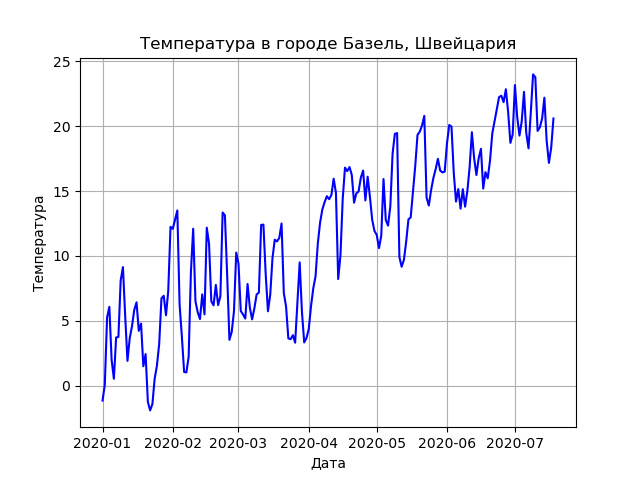
\includegraphics[width=.7\linewidth]{extra/temperature.png}
  \captionof{figure}{Исходные данные}
  \label{fig:prplot}
\end{center}
Для прогнозирования временных рядов была выбрата нейросеть SARIMA (Seasonal ARIMA). ARIMA является одной из самый популярных нейросетей для анализа временных рядов на Python, а сезонная природа температуры подталкивает к использованию сезонной версии.\\
Данные были взяты с сайта meteoblue.com. Так как данные были взяты с избытком, а также потому что сайт предоставляет данные по часам данные следует подготовить.
\begin{lstlisting}[language=Python, caption=Подготовка данных]
import pandas as pd
import numpy as np
from matplotlib import pyplot as plt
import statsmodels.api as sm
from statsmodels.tsa.statespace.sarimax import SARIMAX
from sklearn.metrics import mean_squared_error, mean_absolute_error

dataset = pd.read_csv('weather_data.csv', header=0, parse_dates=['datetime'])

dataset = dataset.set_index('datetime').resample("d").mean().asfreq('d')

df = dataset.iloc[:200,:]
\end{lstlisting}
% -------------------
Параметрами для модели являются параметры AR (autoregressive) он же p, I (integration) он же d, MA (moving average) он же q, а также аналогичные сезонные параметры P, D, Q и m - количество временных шагов в одном сезоне. Параметр d - сколько нужно продифференцировать ряд, чтобы он стал стационарен,а все остальные параметры примерно можно узнать коррелограммы. Получить параметры можно с помощью следующего кода.
\begin{lstlisting}[language=Python, caption=Получение параметров модели]
  test = sm.tsa.adfuller(df['temperature'])
  if test[0]> test[4]['5%']: 
      print('есть единичные корни, ряд не стационарен')
  else:
      print('единичных корней нет, ряд стационарен')
  
  df_diff = df['temperature'].diff(periods=1).dropna()
  test = sm.tsa.adfuller(df_diff)
  if test[0]> test[4]['5%']: 
      print('есть единичные корни, ряд не стационарен')
  else:
      print('единичных корней нет, ряд стационарен')
  
  fig = plt.figure(figsize=(12,8))
  ax1 = fig.add_subplot(211)
  fig = sm.graphics.tsa.plot_acf(df_diff.dropna(), lags=99, ax=ax1)
  plt.grid()
  ax2 = fig.add_subplot(212)
  fig = sm.graphics.tsa.plot_pacf(df_diff.dropna(), lags=99, ax=ax2)
  plt.grid()
  plt.savefig('latex/extra/acf_pacf.png')
  plt.show()
\end{lstlisting}
\begin{lstlisting}[style=text, caption=Вывод кода из листинга 2]
  есть единичные корни, ряд не стационарен
  единичных корней нет, ряд стационарен
\end{lstlisting}
\begin{center}
  \centering
  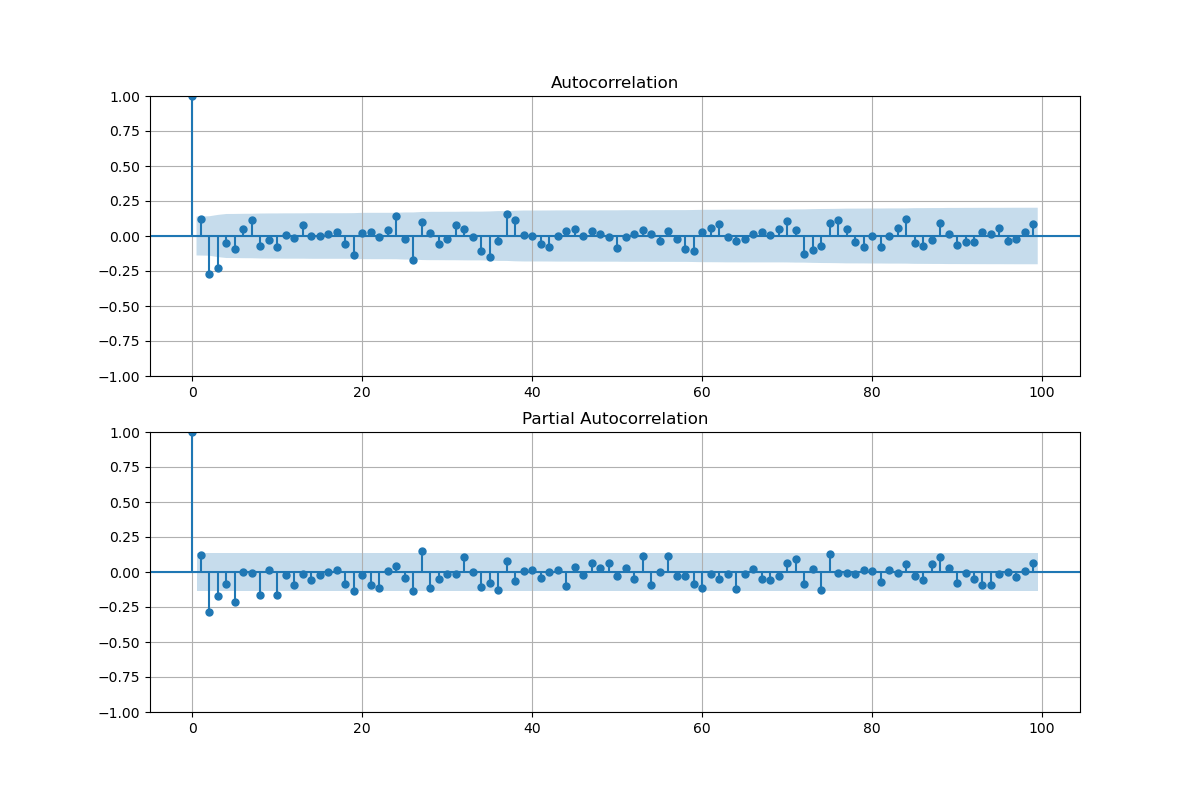
\includegraphics[width=1\linewidth]{extra/acf_pacf.png}
  \captionof{figure}{коррелограммы}
  \label{fig:prplot}
\end{center}
% -------------------
Как видно из текстового вывода d=1. \\
Из коррелограммы p=3, q=2, m=8. Т.к. первый сущещственный лаг на коррелограмме отрицательный P=0, Q=2. Параметры получены, следующий шаг - обучение модели.
\begin{lstlisting}[language=Python, caption=Обучение модели и прогноз на продолжительный срок]
  df.reset_index()

  train = df.iloc[:-50,:]
  test = df.iloc[-50:,:]
  
  model = SARIMAX(train, order=(3, 1, 2), seasonal_order=(0, 0, 2, 8))
  model_fit = model.fit()
  
  fcast_len = len(test)
  fcast = model_fit.forecast(fcast_len)
  
  mse = mean_squared_error(test, fcast)
  rmse = np.sqrt(mse)
  mae = mean_absolute_error(test, fcast)
  
  print(f'Mean Squared Error: {mse}')
  print(f'Root Mean Squared Error: {rmse}')
  print(f'Mean Absolute Error: {mae}')
  
  plt.title('Температура в городе Базель, Швейцария')
  plt.plot(train, label='Train')
  plt.plot(fcast, label='Forecast')
  plt.plot(test, label='Test')
  plt.xlabel('Дата')
  plt.ylabel('Температура')
  plt.grid()
  plt.legend()
  plt.savefig('latex/extra/prediction.png')
  plt.show()
\end{lstlisting}
\begin{lstlisting}[style=text, caption=Процесс обучения модели]
RUNNING THE L-BFGS-B CODE

  * * *

Machine precision = 2.220D-16
N =            8     M =           10
This problem is unconstrained.

At X0         0 variables are exactly at the bounds

At iterate    0    f=  2.38436D+00    |proj g|=  3.14481D-01

At iterate    5    f=  2.26655D+00    |proj g|=  7.15151D-02

At iterate   10    f=  2.25628D+00    |proj g|=  2.08637D-03

At iterate   15    f=  2.25627D+00    |proj g|=  4.10184D-04

At iterate   20    f=  2.25626D+00    |proj g|=  5.49808D-04

  * * *

Tit   = total number of iterations
Tnf   = total number of function evaluations
Tnint = total number of segments explored during Cauchy searches
...
CONVERGENCE: REL_REDUCTION_OF_F_<=_FACTR*EPSMCH
\end{lstlisting}
\begin{center}
  \centering
  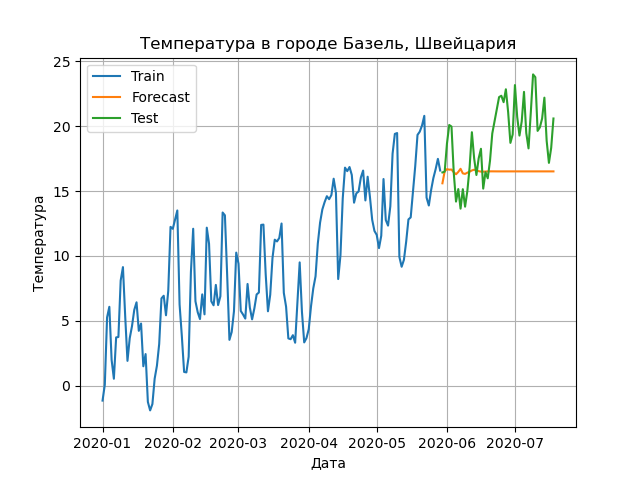
\includegraphics[width=.7\linewidth]{extra/prediction.png}
  \captionof{figure}{Результат предсказания модели}
  \label{fig:prplot}
\end{center}
\begin{lstlisting}[style=text, caption=Отклонения результатов модели]
  Mean Squared Error: 12.876863306757866
  Root Mean Squared Error: 3.5884346596751437
  Mean Absolute Error: 2.9688323338931313
\end{lstlisting}
% -------------------
Как видно по графику чем дальше он начальных условий, тем хуже предсказание. Причиной служит очень большие колебания температур в близкие даты. Для корректировки модели воспользуемся скользящим прогнозом и, чтобы не усложнять задачу, пронозировать будем на один шаг вперёд, после чего корректировать.
\begin{lstlisting}[language=Python, caption=Использование скользящего прогноза]
  def rolling_forecast(train, test, order, season):
  history = train.iloc[:,:].asfreq('d')
  model = SARIMAX(history, order=order, seasonal_order=season)
  model_fit = model.fit(disp=False)
  predictions = []
  results = {}
  yhat = model_fit.forecast()

  predictions.append(yhat)
  history = pd.concat([history, pd.DataFrame([test.iloc[0,:]])]).asfreq('d')
  for i in range(1, len(test)):
      model = SARIMAX(history, order=order, seasonal_order=season)
      model_fit = model.fit(disp=False)
      yhat = model_fit.forecast()
      predictions.append(yhat)
      history = pd.concat([history, pd.DataFrame([test.iloc[i,:]])]).asfreq('d')
  mse = mean_squared_error(test, predictions)
  mae = mean_absolute_error(test, predictions)
  rmse = np.sqrt(mse)
  predictions = pd.Series(predictions, index=test.index)
  results['predictions'] = predictions
  results['mse'] = mse
  results['rmse'] = rmse
  results['mae'] = mae
  return results

rolling_fcast = rolling_forecast(train, test, (2, 1, 3), (0, 0, 2, 8))

print(f'Mean Squared Error: {rolling_fcast["mse"]}')
print(f'Root Mean Squared Error: {rolling_fcast["rmse"]}')
print(f'Mean Absolute Error: {rolling_fcast["mae"]}')

plt.title('Температура в городе Базель, Швейцария')
plt.plot(train, label='Train')
plt.plot(rolling_fcast['predictions'], label='Forecast')
plt.plot(test, label='Test')
plt.xlabel('Дата')
plt.ylabel('Температура')
plt.grid()
plt.legend()
plt.savefig('latex/extra/rolling_prediction.png')
plt.show()
\end{lstlisting}
\begin{center}
  \centering
  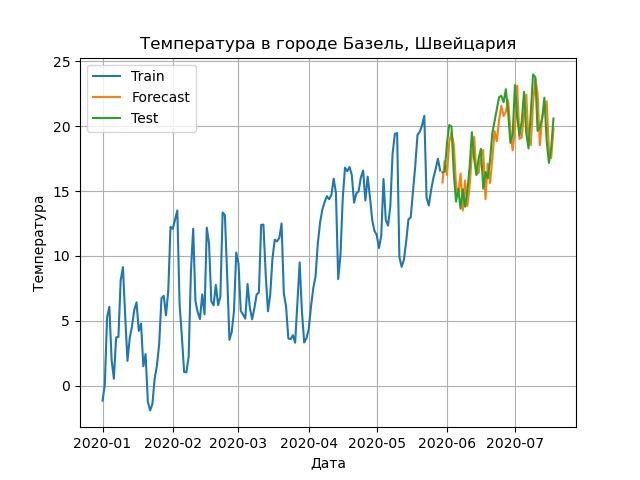
\includegraphics[width=.7\linewidth]{extra/rolling_prediction.png}
  \captionof{figure}{Результат предсказания модели с использованием скользящего прогноза}
  \label{fig:prplot}
\end{center}
\begin{lstlisting}[style=text, caption=Отклонения результатов модели с использованием скользящего прогноза]
  Mean Squared Error: 2.885728192709077
  Root Mean Squared Error: 1.6987431214604158
  Mean Absolute Error: 1.468788413247244
\end{lstlisting}
Как видно по графику и значениям ошибок модель стала достаточно точно предсказывать температуру на следующий день.
\newpage
% -------------------------------------------------------
\section{Ответы на вопросы}
\subsection*{Вопросы}
\begin{enumerate}
  \item Приведите примеры временных рядов при создании цифровых двойников;
  \item Что понимают под цифровым двойником эксперта?
  \item В чем состоит задача прогнозирования временных рядов?
  \item Что понимается под реконструкцией математической модели системы? Какова цель реконструкции ММС?
  \item Что такое «переменная состояния» системы? Приведите примеры.
  \item Перечислите основные этапы реконструкции математической модели системы
  \item Как оценить адекватность разработанной модели?
\end{enumerate}
\subsection*{Ответы}
\begin{enumerate}
  \item Примеры временных рядов при создании цифровых двойников включают данные о температуре, давлении, вибрации и скорости вращения в промышленном оборудовании, показания датчиков в реальном времени для мониторинга состояния объектов, а также данные о потреблении энергии, нагрузке или состоянии здоровья в медицинских устройствах.
  \item Цифровой двойник эксперта — это виртуальная модель, которая симулирует знания, опыт и навыки реального специалиста в конкретной области. Такой цифровой двойник может анализировать ситуации, давать рекомендации и принимать решения, имитируя поведение настоящего эксперта, используя данные, алгоритмы и искусственный интеллект.
  \item Задача прогнозирования временных рядов состоит в предсказании будущих значений на основе анализа исторических данных, представленных в виде последовательности измерений, сделанных через равные интервалы времени.
  \item Реконструкция математической модели системы — это процесс создания или восстановления модели, описывающей поведение реальной системы на основе наблюдаемых данных. Это может включать выявление зависимостей, определение параметров модели или корректировку существующих моделей для более точного отображения процессов.  Цель реконструкции ММС заключается в том, чтобы получить адекватное математическое представление системы, которое позволяет точно прогнозировать ее поведение, анализировать различные сценарии и принимать обоснованные решения. Реконструкция важна, когда прямое моделирование невозможно или данные системы неполны.
  \item Переменная состояния системы — это величина, которая полностью описывает состояние системы в определенный момент времени. Она отражает всю необходимую информацию для предсказания будущего поведения системы, если известны все входы и законы её динамики. \\
  Примеры переменных состояния:
  \begin{enumerate}
    \item Температура двигателя
    \item Скорость автомобиля.
  \end{enumerate}
  \item Основные этапы реконструкции математической модели системы включают:
  \begin{enumerate}
    \item Сбор данных
    \item Анализ системы
    \item Выбор типа модели
    \item Идентификация параметров модели
    \item Калибровка модели
    \item Проверка и валидация модели
    \item Использование модели
  \end{enumerate}
  \item Оценить адекватность модели можно сравнив её с реальными данными.
\end{enumerate}
\newpage
%---------------------------------------------------------
\section{Вывод}
При выполнении лабораторной работы была разработана цифровую модель эксперта на основе нейросети SARIMAX, решающая задачу прогнозирования температуры. 
\end{document}
